% 图 51.4 —— 由 `checks/emit_hand.py` 自动拼出（probe 精测 + prims2 图元分解）
%%
% ⚠ 这是**稿子不是成品**：跑 `checks/checkhand.py 51.4` 看指标 + 看叠合图。
%%
%% ⚠ 待核：
%   · 本图 probe 报出阴影族 2 个 —— **本脚本不生成阴影**（要照原书手写）；prims2 的 strokes 里可能含阴影线，核对时留意别画重
%   · 可疑字形 1 项（空心圈 ⊙ 常被认成字母 o）—— 见文件末
%%
\documentclass[12pt]{standalone}
\usepackage{fontspec}
\setsansfont{Arial}
\newfontfamily\mfallback{DejaVu Sans}
\usepackage{tikz}
\usetikzlibrary{arrows.meta}
\begin{document}
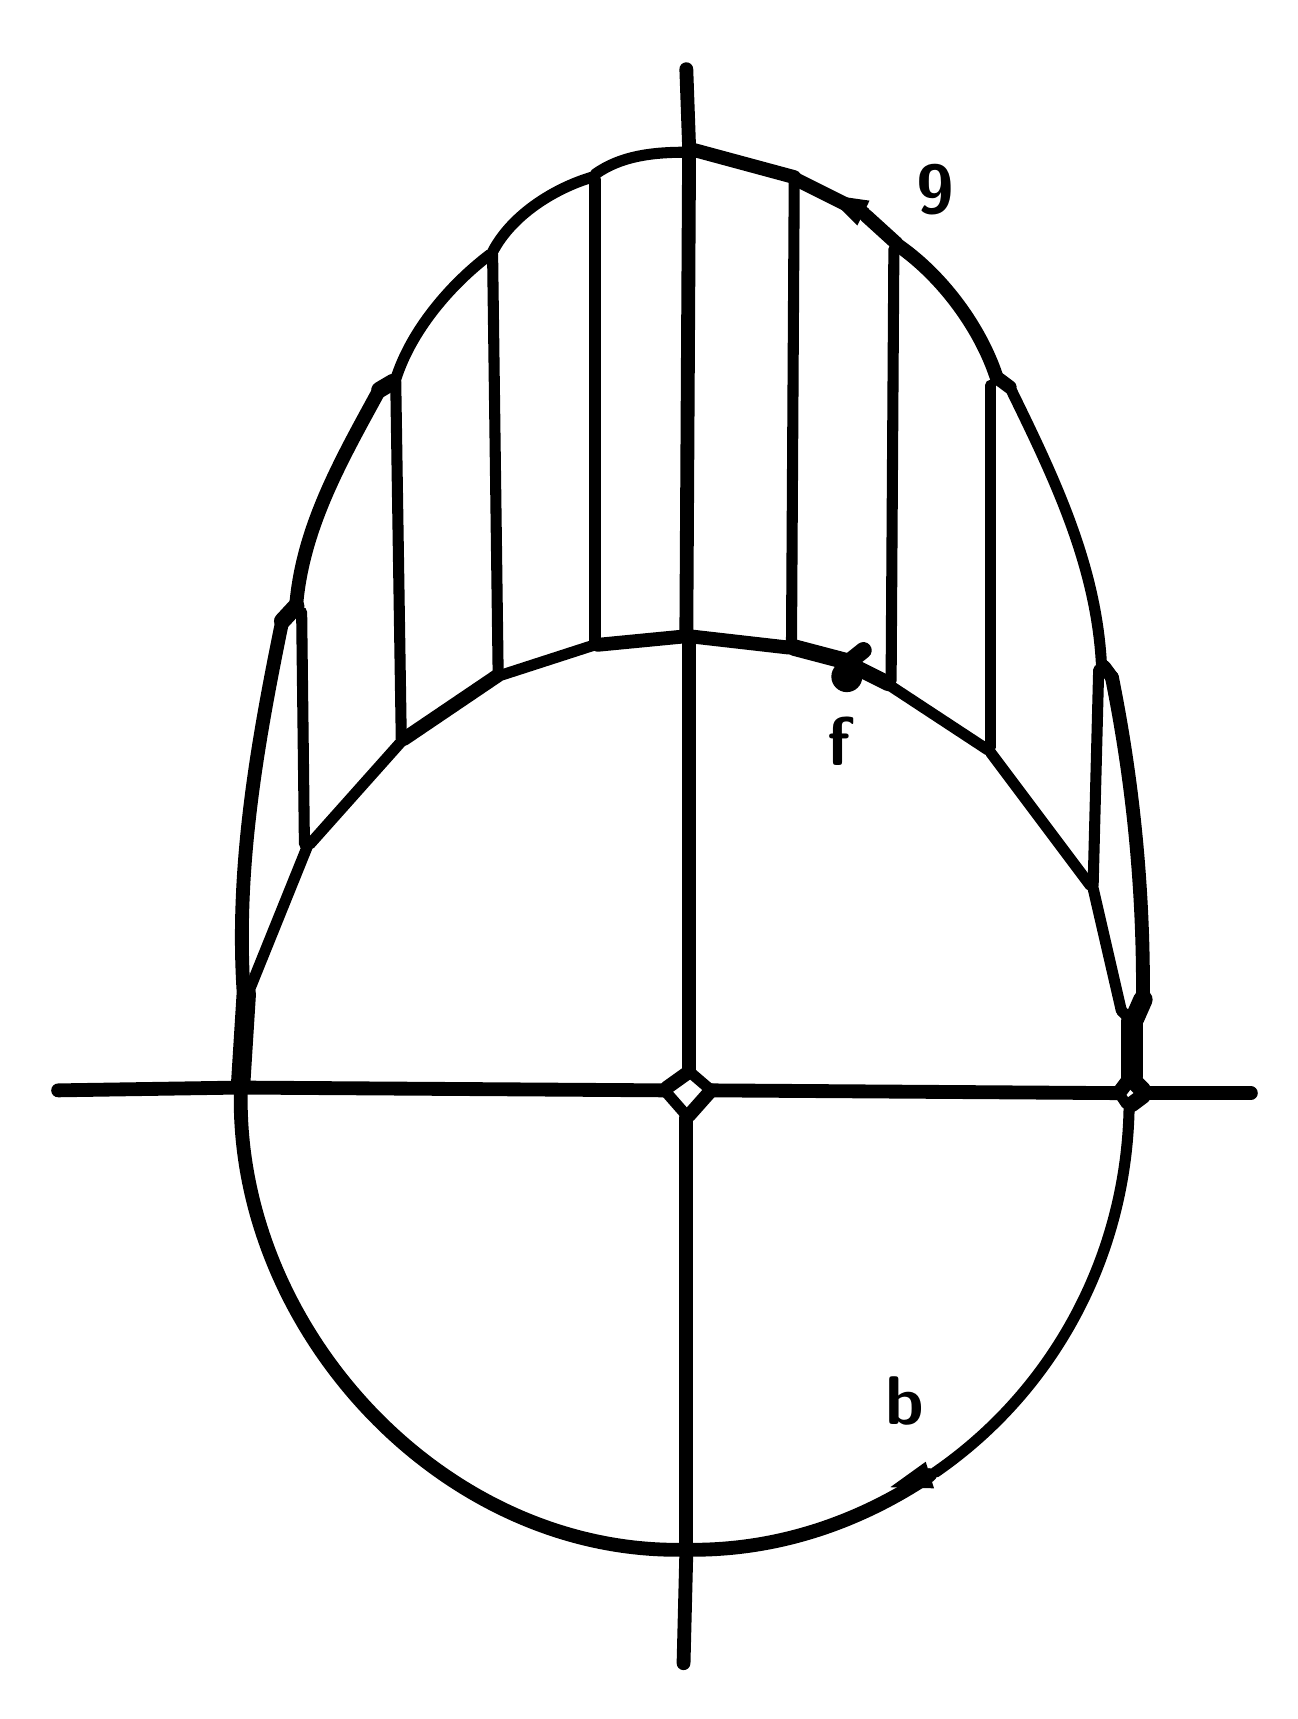
\begin{tikzpicture}[x=1pt, y=-1pt, line width=5.9pt, line cap=round, line join=round]

  %% ════ 填充区（prims2 的 fills）════

  %% ════ 直线段（prims2 的 strokes）════
  \draw[line width=5.9pt] (127.1,130.9) -- (132.0,128.0);
  \draw[line width=6.0pt] (97.0,209.0) -- (92.0,214.4);
  \draw[line width=3.0pt] (97.0,209.0) -- (99.0,211.2);
  \draw[line width=4.0pt] (99.0,211.2) -- (100.0,295.0);
  \draw[line width=5.0pt] (231.0,383.0) -- (238.0,378.0);
  \draw[line width=5.0pt] (238.0,219.0) -- (239.0,46.0);
  \draw[line width=4.0pt] (101.0,296.0) -- (80.0,348.0);
  \draw[line width=6.0pt] (277.0,224.0) -- (296.0,229.0);
  % （略）线段 (308.0,63.0)-(303.0,67.0) 线宽6.5 —— 是箭头头那一坨，已由箭头头代替
  \draw[line width=5.0pt] (238.0,549.0) -- (238.0,394.0);
  \draw[line width=4.0pt] (102.0,295.0) -- (135.0,258.0);
  \draw[line width=5.0pt] (404.0,385.0) -- (442.0,385.0);
  \draw[line width=4.0pt] (347.0,261.0) -- (312.0,238.0);
  \draw[line width=4.0pt] (205.0,55.0) -- (205.0,222.0);
  \draw[line width=4.0pt] (168.0,82.0) -- (170.0,233.0);
  \draw[line width=5.0pt] (238.0,551.0) -- (237.0,591.0);
  \draw[line width=5.0pt] (278.0,55.0) -- (302.0,67.0);
  \fill (304.2,62.5) -- (299.8,71.5) -- (288.6,60.3) -- cycle;
  \draw[line width=4.0pt] (385.0,310.0) -- (387.0,232.0);
  \draw[line width=4.0pt] (276.0,223.0) -- (277.0,55.0);
  \draw[line width=5.0pt] (230.0,384.0) -- (79.0,383.0);
  \draw[line width=4.0pt] (133.0,128.0) -- (135.0,257.0);
  \draw[line width=4.9pt] (351.0,127.0) -- (354.9,129.9);
  \draw[line width=4.0pt] (205.0,223.0) -- (171.0,234.0);
  \draw[line width=5.7pt] (403.0,386.0) -- (399.0,389.0);
  \draw[line width=6.1pt] (399.0,380.0) -- (403.0,384.0);
  \draw[line width=7.0pt] (77.0,381.0) -- (79.0,349.0);
  \draw[line width=5.0pt] (314.0,78.0) -- (303.0,68.0);
  \draw[line width=5.0pt] (277.0,54.0) -- (240.0,44.0);
  \draw[line width=4.0pt] (398.0,358.0) -- (395.2,355.2);
  \draw[line width=4.0pt] (395.2,355.2) -- (385.0,311.0);
  \draw[line width=5.0pt] (394.0,385.0) -- (247.0,384.0);
  % （略）线段 (326.0,515.0)-(327.0,522.0) 线宽8.1 —— 是箭头头那一坨，已由箭头头代替
  \draw[line width=3.8pt] (397.0,389.0) -- (395.0,386.0);
  \draw[line width=5.0pt] (239.0,393.0) -- (247.0,384.0);
  \draw[line width=5.5pt] (297.0,230.0) -- (311.0,237.0);
  \draw[line width=7.0pt] (400.0,358.0) -- (403.0,351.2);
  \draw[line width=4.9pt] (391.8,234.8) -- (389.0,231.0);
  \draw[line width=5.0pt] (239.0,221.0) -- (239.0,377.0);
  \draw[line width=8.0pt] (399.0,359.0) -- (399.0,379.0);
  \draw[line width=5.0pt] (240.0,220.0) -- (275.0,224.0);
  \draw[line width=4.0pt] (312.0,236.0) -- (313.0,80.0);
  \draw[line width=5.0pt] (136.0,257.0) -- (170.0,234.0);
  \draw[line width=3.0pt] (350.0,127.0) -- (348.0,129.2);
  \draw[line width=4.0pt] (348.0,129.2) -- (348.0,260.0);
  \draw[line width=5.0pt] (239.0,43.0) -- (238.0,15.0);
  \draw[line width=5.0pt] (206.0,223.0) -- (237.0,220.0);
  \draw[line width=4.0pt] (384.0,310.0) -- (348.0,262.0);
  \draw[line width=4.0pt] (231.0,385.0) -- (238.0,393.0);
  \draw[line width=4.0pt] (247.0,384.0) -- (240.0,378.0);
  \draw[line width=6.0pt] (297.0,229.0) -- (302.0,225.0);
  \draw[line width=5.2pt] (398.0,380.0) -- (395.0,384.0);
  \draw[line width=5.0pt] (11.0,384.0) -- (76.0,383.0);

  %% ════ 曲线（prims2 的 curves —— 三段式，坐标同为 (y,x)）════
  \draw[line width=5.0pt] (97.0,209.0) .. controls (99.3,180.4) and (113.6,155.7) .. (127.1,130.9);
  \draw[line width=5.0pt] (92.0,214.4) .. controls (83.2,257.4) and (75.1,302.4) .. (78.0,348.0);
  \draw[line width=5.0pt] (237.0,550.0) .. controls (149.9,551.5) and (75.5,470.5) .. (77.0,385.0);
  \draw[line width=5.0pt] (239.0,550.0) .. controls (270.8,550.3) and (300.4,540.2) .. (326.0,523.0);
  \fill (324.5,518.2) -- (327.5,527.8) -- (311.7,527.4) -- cycle;
  \draw[line width=5.0pt] (350.0,126.0) .. controls (344.1,108.3) and (330.7,90.1) .. (315.0,79.0);
  \draw[line width=4.0pt] (354.9,129.9) .. controls (370.5,161.8) and (386.1,193.8) .. (388.0,230.0);
  \draw[line width=4.0pt] (328.0,522.0) .. controls (372.0,491.6) and (397.2,442.2) .. (398.0,390.0);
  \draw[line width=4.0pt] (238.0,45.0) .. controls (226.2,45.0) and (214.4,46.2) .. (205.0,53.0);
  \draw[line width=4.0pt] (204.0,54.0) .. controls (190.2,58.1) and (174.9,67.7) .. (168.0,81.0);
  \draw[line width=4.0pt] (167.0,82.0) .. controls (152.4,93.1) and (138.5,109.6) .. (133.0,127.0);
  \draw[line width=5.0pt] (403.0,351.2) .. controls (403.3,311.2) and (399.4,272.5) .. (391.8,234.8);

  %% ════ 实心点 ════
  % （略）(299.3,71.3) r=4.6 落在箭头头上 —— 已由箭头头代替
  \fill (296.0,234.5) circle (5.6);
  % （略）(329.0,524.5) r=5.3 落在箭头头上 —— 已由箭头头代替

  %% ════ 标签（probe 直接给的 \node 行）════
  %% ⚠ 全部补了 fill=white：文字在最上层，否则与曲线交叉干扰
     \node[anchor=center,inner sep=0pt,fill=white,font=\fontsize{34.8}{43.5}\selectfont] at (328.0,58.4) {\textsf{\textbf{9}}};   % box(317,46,18,23)
     \node[anchor=center,inner sep=0pt,fill=white,font=\fontsize{29.1}{36.4}\selectfont] at (294.0,258.0) {\textsf{\textbf{\textit{f}}}};   % box(288,246,11,23)
     \node[anchor=center,inner sep=0pt,fill=white,font=\fontsize{30.0}{37.5}\selectfont] at (316.8,496.2) {\textsf{\textbf{\textit{b}}}};   % box(307,484,17,22)

  % 钉死画布：否则超出的图元/控制点会把页面撑大，1:1 回比就失准
  \pgfresetboundingbox
  \path[use as bounding box] (0,0) rectangle (449,601);
\end{tikzpicture}
\end{document}

% ⚠ 待核清单（probe 拿不准，人眼过一遍）：
%   · 未识别/跳过：⑤ 跳过/未识别的字形
